\chapter{System Environment and Protocol Designs}
\label{cha:3_design}
\parskip=0ex

\indent This chapter describes the assumptions used in this thesis, an overview on Skipchain technology, the proposed system architecture design and the proposed protocol design. All assumptions used in the proposed firmware update framework is described in Section~\ref{sec:1_assumptions}. An overview of Skipchain technology is explained in Section~\ref{sec:2_overview}. The system architecture design and the proposed protocol design for the firmware update mechanism are explained in Section~\ref{sec:3_architectureDesign} and Section~\ref{cha:4_protocoldesign}, respectively.

\section{Assumptions}
\label{sec:1_assumptions}

The assumptions used in this thesis are listed as follows:
\begin{enumerate}
	\item The proposed firmware update mechanism uses push-update method, in which the vendor repository sends the metadata of a new firmware in the form of smart contract to the skipchain network. Once the corresponding smart contract is verified, all the nodes in the skipchain network will synchronize their smart contract data with the latest data.
	\item  In the proposed scenario, the gateway as a passive node in the skipchain network will obtain a notification on the newly released firmware from the verified smart contract. Afterward, the gateway will check if the newly released firmware is required by the IoT devices connected to it.
	\item The scope of IoT devices in this thesis have low-power consumption, small storage capacity, limited computation capability, and limited Internet connectivity. However, the IoT devices are able to perform simple Hash computation and simple value comparison.
	\item The IoT devices have pre-installed the public key of vendor to authenticate the firmware signature.
	\item Each IoT device have pre-installed a small portion of skipchain data to allow the associated gateway to join a specific skipchain network. In addition, the pre-installed skipchain data enable the IoT device to securely verify the more recent skipchain data from the associated gateway.
	\item The firmware binary is distributed from the vendor repository to the targeted IoT device through a secure channel.
	\item The vendor repository and the corresponding vendor node are communicating through a non-secure communication channel.
	\item The peer-to-peer connection between gateway and IoT devices is not in secure channel.
\end{enumerate}

\section{Skipchain Overview}
\label{sec:2_overview}

Skipchain is a cryptographically traversable, offline and p2p verifiable blockchain structure~\cite{Skipchain}. Skipchain implements the concept of skiplist into a blockchain structure by adding long-distance forward and backward links. The long-distance backward link has been introduced in Chainiac~\cite{chainiac}. The long-distance backward link contains a hashed-address of the previously created block. This backward link allows users to trace a transaction history starting from the latest block data. The transaction trace feature could be performed when the user's device contains more recent block data than the block data of searched transaction.

The unique forward link in skipchain structure enables user to verify transaction history even when the user's blockchain data is behind the more recent blockchain data. This forward link contains two pieces of information as follow:
\begin{enumerate}
	\item A secure hash-pointer to the first block committed by the next consensus group.
	\item A description of how the consensus group has changed, such as which cosigner joins or leaves the consensus group (indicated by the addition or reduction on the number of cosigner's public keys).
\end{enumerate}
Once the successor of a block is committed, the consensus group responsible for the block creates and collectively signs a forward link. This process is similar to securely issues an information of the current consensus group's members for the prior, already-committed block. The security of forward link is assured by a collective signature.

Skipchain uses a tree-based collective signing (CoSi)~\cite{cosigning} schemes, in which each signer (\textit{cosigner}) joins the Schnorr signature~\cite{schnorrsign} to agree on a valid statement. The group of cosigner, known as collective authority (cothority), will perform the consensus-like process where each cosigner will verify and sign a valid transaction. The CoSi architecture is illustrated in Figure~\ref{fig:cothority}. In the CoSi architecture, each record could be collectively signed by different cothority member.
\begin{figure}[H]
	\begin{center}
		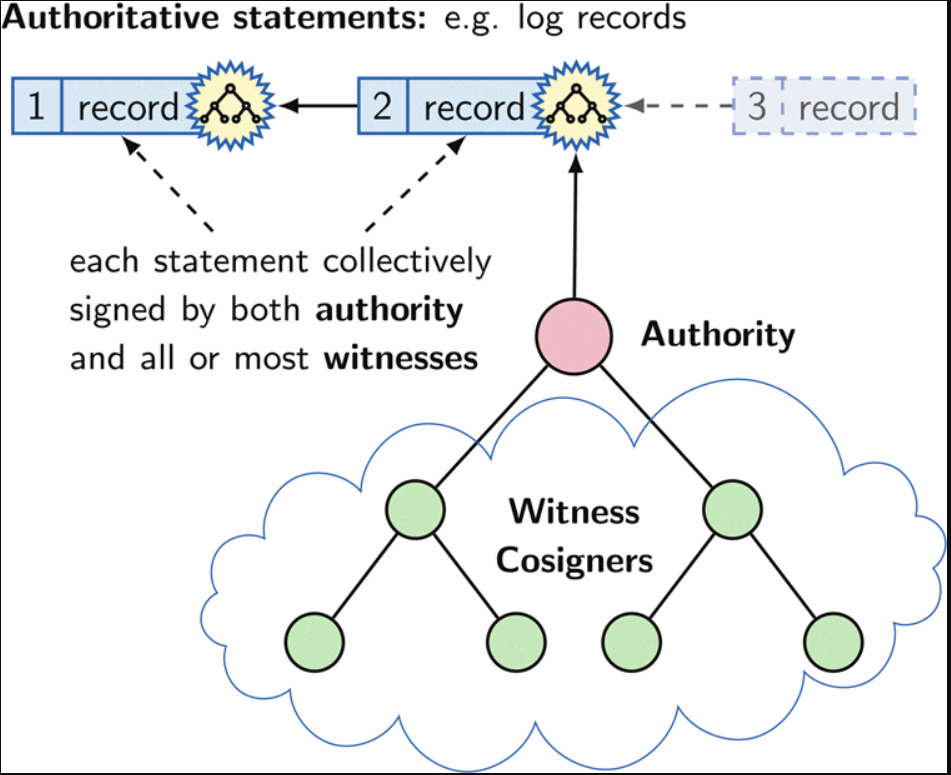
\includegraphics[width=1.0\textwidth]{figures/cosigning.png}
		\caption{CoSi protocol architecture~\cite{cosigning}} 
		\label{fig:cothority}
	\end{center}
\end{figure}

As the forward links are signed by different cothority members, the user could securely perform forward tracing on the more recent blockchain data without having to trust the other parties. In addition, the user could learn all the changes on the consensus group and would be able to know the correct set of public keys while performing the forward tracing. The set of public keys will be used to verify the corresponding collective signatures in the blockchain. Since all of the forward links are collectively signed by cothority members, an attacker can not create a fake blockchain branch unless the attacker compromises or colludes with large number of cothority members.

\section{Architecture Design}
\label{sec:3_architectureDesign}

In this thesis, we proposed the skipchain-based firmware update framework for IoT environments. The architecture of our framework is illustrated in Figure~\ref{fig:1_fotb}. There are three roles in the architecture design, described as follow:
~\begin{enumerate}
	\item Vendor: the manufacturer of the specific IoT device and acts as active node in the skipchain network. The active node in the skipchain network is actively do the verification process as a Cothority's member. Each time a vendor pushes a new version of firmware, the vendor repository needs to broadcast the vendor-signed firmware metadata to the Cothority nodes via the vendor's active node.
	\item Gateway: the gateway for connected IoT devices and connected to the skipchain network as passive node. The passive node in skipchain network does not participate in any verification process, however, it only synchronizes the block data with the most recent block data in the skipchain network.
	\item IoT device: the sensor-embedded device that connects to a specific gateway and does not need to fully trust the gateway device. Each IoT device can verify the notification of firmware update from the gateway by using its pre-installed skipchain data.
\end{enumerate}

\begin{figure}[H]
	\begin{center}
		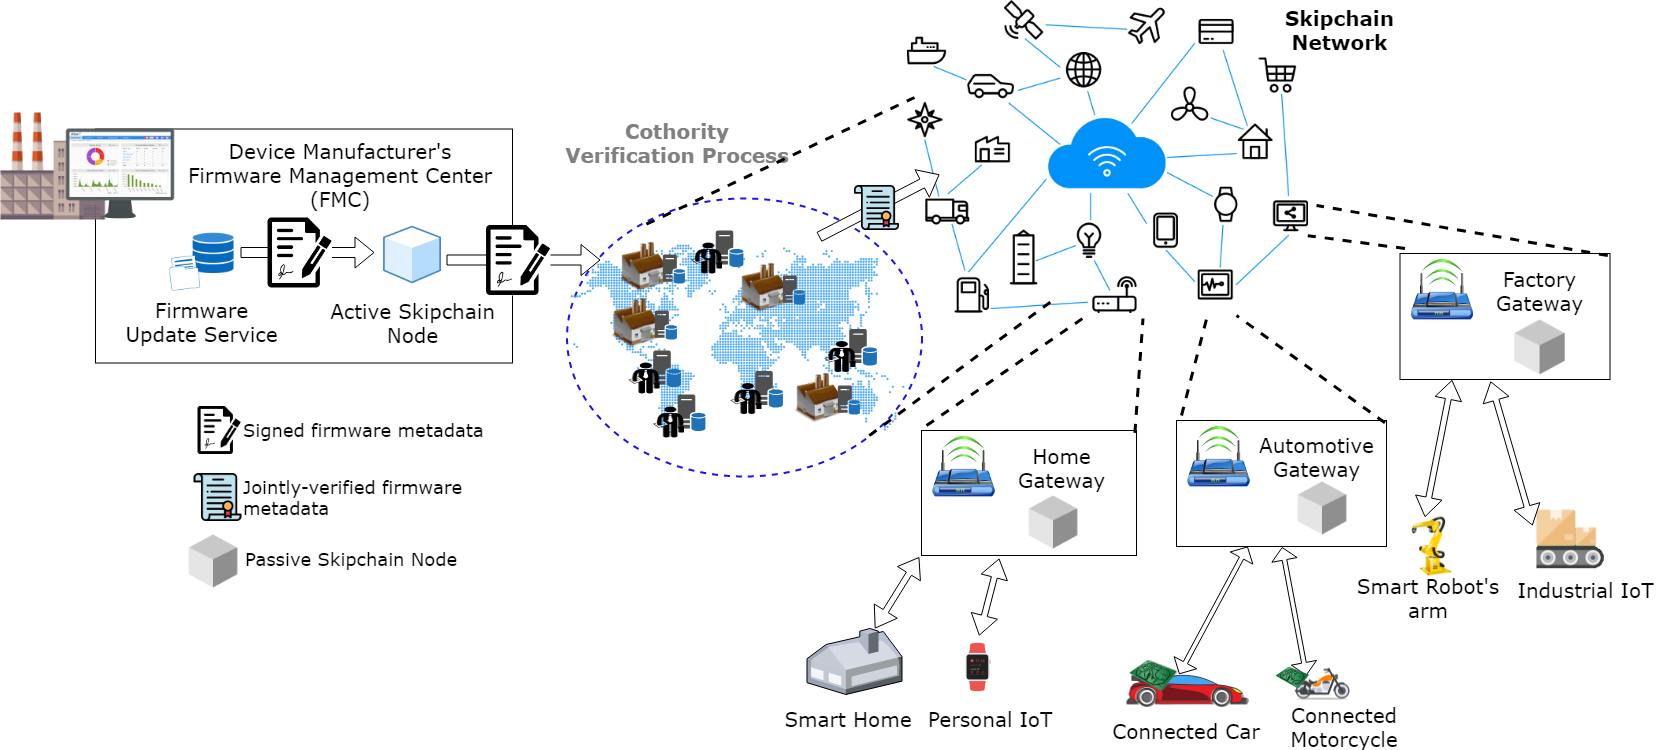
\includegraphics[width=1.0\textwidth]{figures/firmware_update-skipchain-based_fotb.png}
		\caption{Firmware Over-the-Skipchain (FOTS) process diagram} 
		\label{fig:1_fotb}
	\end{center}
\end{figure}

From the Figure~\ref{fig:1_fotb}, there are two kinds of node in the skipchain network namely: active node and passive node. The active nodes are actively performing the verification process on any new smart contract data containing the metadata of a new version of firmware. In addition, the active node acts as Cothority's member in the proposed skipchain network. In the contrary to the active node, the passive node only continuously synchronizes the block data with the more recent block data in the skipchain network and does not involve in any verification process of a newly released smart contract. Each gateway in the proposed architecture design manages at least one IoT device in local network environment. For example, there are smart home appliances and personal IoT devices connected to a home router as gateway. The connection between the gateway and the IoT device is peer-to-peer connection, such as Bluetooth connection.

\begin{figure}[H]
	\begin{center}
		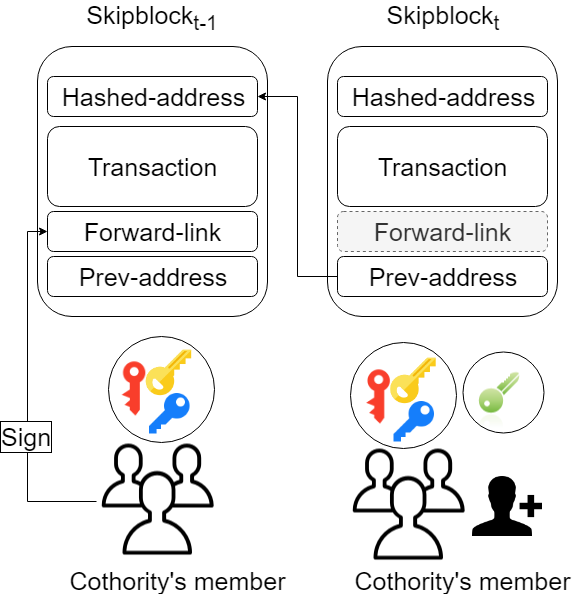
\includegraphics[width=1.0\textwidth]{figures/firmware_update-skipblock-diagram.png}
		\caption{Skipblock structure diagram} 
		\label{fig:skipblock_diagram}
	\end{center}
\end{figure}

The skipblock structure as shown in Figure~\ref{fig:skipblock_diagram}, consists of four main contents: hashed-address, transaction, forward link, and prev-address. These four contents are described as follow:
~\begin{enumerate}
	\item Hashed-address: a hashed-value that is unique and will be the address for a skipblock. Each skipblock is accessible through this hashed-address.
	\item Transaction: the transaction contains the metadata of a firmware, such as the targeted device model, the firmware version, and the url to download the corresponding firmware binary in the vendor repository. A skipblock could contain one or more transaction data.
	\item Forward Link: the unique structure from skipchain itself, it contains the next block's address and the difference of the current cothority's members that verify the $skipblock_t$. The cothority's members those verify the $skipblock_{t-1}$ (red, yellow and blue key) need to sign the forward link. In Figure~\ref{fig:skipblock_diagram}, the forward link will contain the information about the new cothority's member with the green key. Later, client will check the forward link, and know which keys do the client need to use to verify the skipblock. And the dashed-line forward link in $skipblock_t$ means that it contain no information of the next block since $t$ is the newest block.
	\item Prev-address: the hashed-address of a previous skipblock.
\end{enumerate}

\begin{figure}[H]
	\begin{center}
		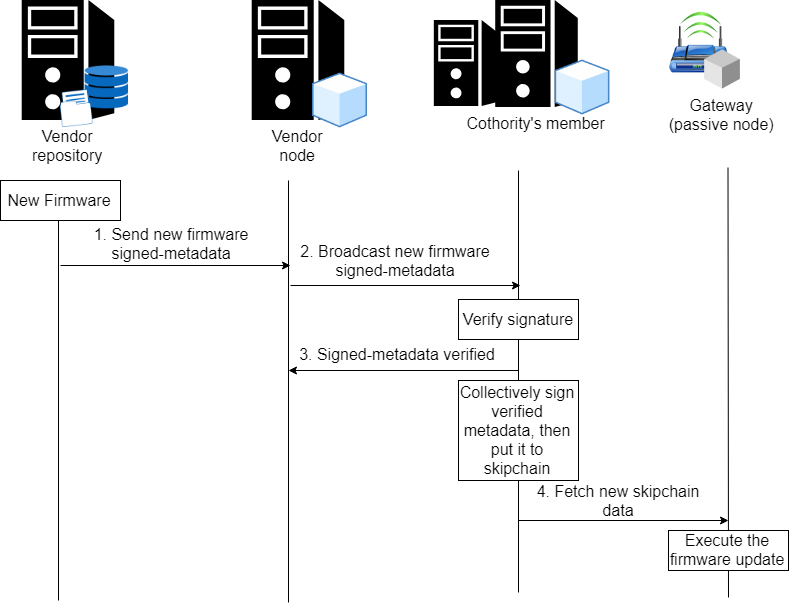
\includegraphics[width=1.0\textwidth]{figures/firmware_update-Firmware_verification_process.png}
		\caption{Firmware update verification process} 
		\label{fig:verificationprocess}
	\end{center}
\end{figure}

In our proposed scheme, we divide the overall process into two parts. The first part is firmware verification process, in which this process will leverage how the metadata of a new version of firmware is verified and how to store the corresponding metadata into the skipchain. After the metadata of the corresponding firmware is sent to the skipchain network, the peer-to-peer verification process will begin. Afterward, the IoT device verifies the firmware update notification from the gateway (in a peer-to-peer connection) before the firmware update is performed by the IoT device.

The firmware verification process of the proposed framework is shown in Figure~\ref{fig:verificationprocess} and described as follow:
~\begin{enumerate}
	\item Each time a vendor releases a new version of firmware, the vendor uses his private key to sign the metadata of the newly released firmware. The metadata of a firmware contains information such as the url to download the corresponding firmware, the version of a firmware, the targeted device model, and other detailed information which will be discussed in Section~\ref{cha:4_protocoldesign}.
	\item The vendor node broadcasts the signed-metadata to the other cothority member to be verified using the corresponding vendor's public key.
	\item After the verification process for the firmware metadata, the cothority will collectively sign the valid metadata and store the signed firmware metadata into the skipblock in the skipchain network.
	\item The gateway as a passive node will continuously synchronize with the skipchain network to fetch the new firmware update information and execute the firmware update mechanism.
\end{enumerate}

The firmware update peer-to-peer verification process is illustrated in Figure~\ref{fig:executionprocess}. After obtaining the firmware update notification, the gateway checks the targeted device model for the firmware update from the newly created skipblock. Afterward, the gateway will notify the corresponding connected IoT devices. Then, the IoT device can verify if the updated firmware comes from the valid skipblock and whether the firmware is published by the correct vendor. After the updated firmware is verified, the IoT device sends its current firmware version to the gateway. Upon receiving the installed firmware version from the IoT device, the gateway will check whether the installed version of firmware is older than the new version of firmware recorded in the skipblock. In the case that the installed firmware version in the IoT device is older than the firmware version in the skipblock, then the gateway will download the new version of firmware binary from the url provided in the metadata. The downloaded firmware binary is sent to the corresponding IoT device to be verified and installed to the device.

\begin{figure}[H]
	\begin{center}
		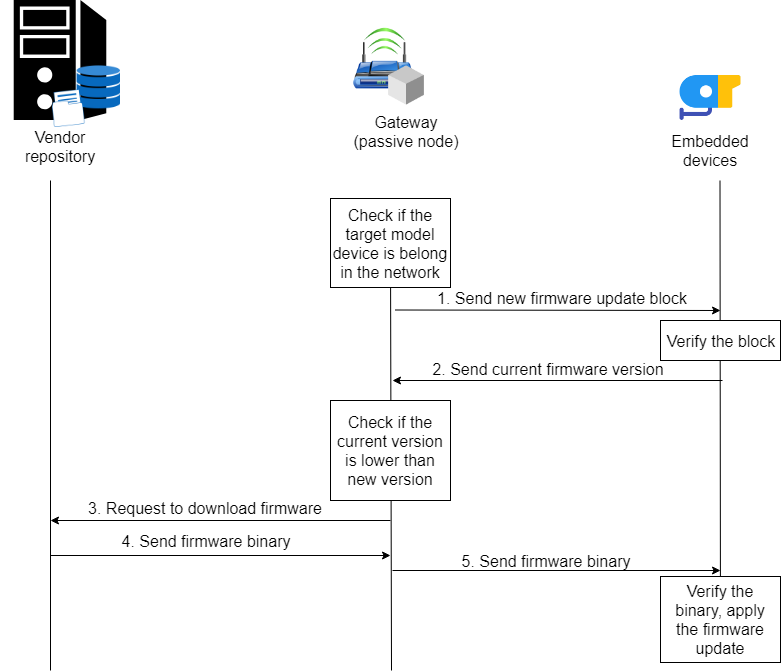
\includegraphics[width=1.0\textwidth]{figures/firmware_update-firmware_update_execution.png}
		\caption{Firmware update peer-to-peer verification process} 
		\label{fig:executionprocess}
	\end{center}
\end{figure}

In the peer-to-peer verification process, the IoT device uses the skipchain's forward link to securely verify the new version of firmware without synchronizing and storing any additional data. Instead, the gateway as a more capable device with more storage capacity and more stable Internet connection can do the synchronization process. The peer-to-peer verification also helpful when a gateway is not connected to the Internet because the offline-gateway can get the firmware update notification from another online-gateway via peer-to-peer notification. In such case, the offline-gateway is still able to verify the new firmware update notification and does not blindly trust the online-gateway. The peer-to-peer verification process is illustrated in Figure~\ref{fig:p2pverification}

\begin{figure}[H]
	\begin{center}
		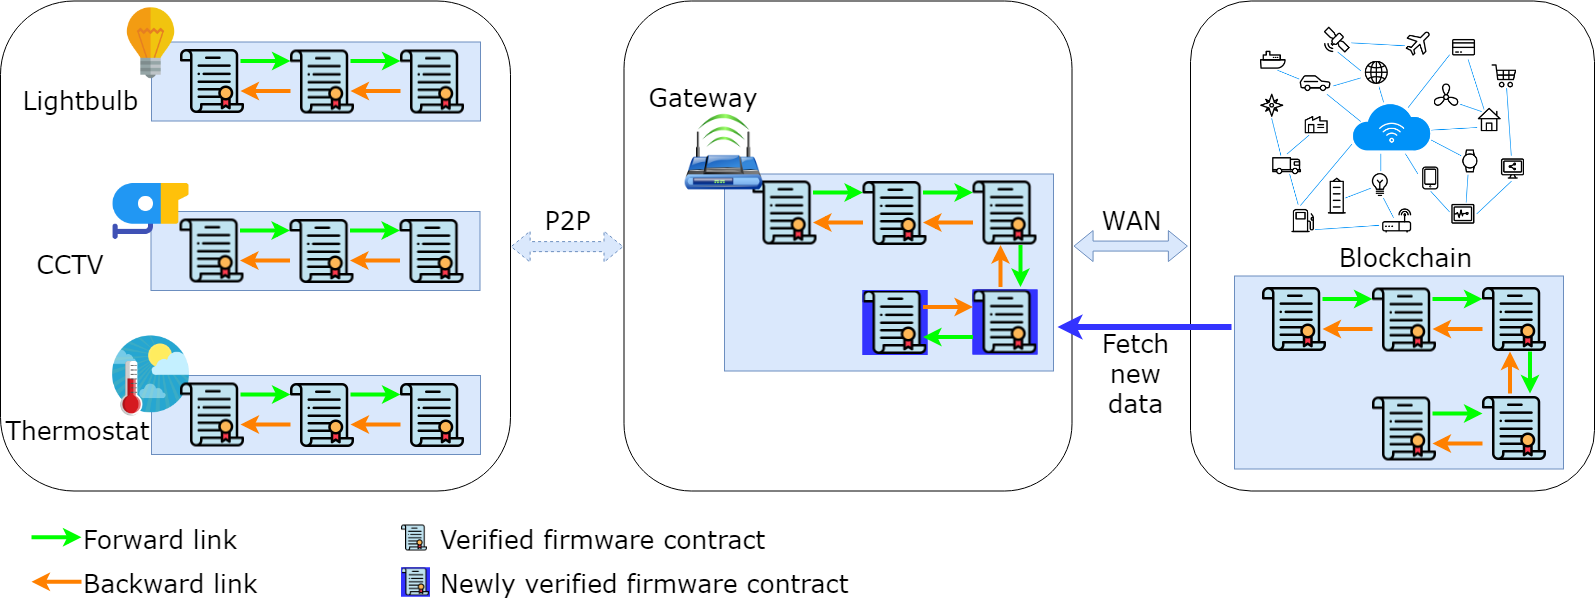
\includegraphics[width=1.0\textwidth]{figures/firmware_update-skipchain_p2p_update.png}
		\caption{Peer-to-peer verification process} 
		\label{fig:p2pverification}
	\end{center}
\end{figure}

In the peer-to-peer verification process, the pre-installed skipblock in the IoT device takes an important role as it contains several valid skipblocks data. The pre-installed skipblock structure is illustrated in Figure~\ref{fig:preinstalled}. In addition, the pre-installed skipblocks contain list of public keys (illustrated by the red, yellow and blue keys in the Figure~\ref{fig:preinstalled}) to verify the given forward link via peer-to-peer connection.

\begin{figure}[H]
	\begin{center}
		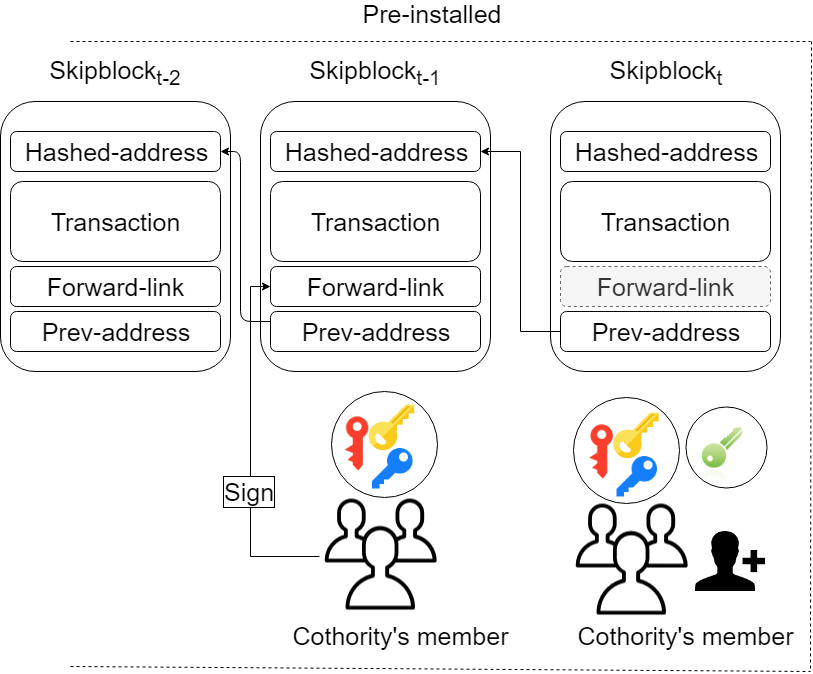
\includegraphics[width=1.0\textwidth]{figures/firmware_update-preinstalled_skipblock.png}
		\caption{Pre-installed skipblock diagram} 
		\label{fig:preinstalled}
	\end{center}
\end{figure}

\section{Protocol Design}
\label{cha:4_protocoldesign}

In this section, our proposed firmware update protocol is introduced and explained. There are two stages of verification before the firmware binary is executed in the proposed protocol: firmware update verification process and peer-to-peer verification process between IoT device and gateway. Table \ref{tab:notation} shows the notations that we use in our protocol.

\begin{table}[H]
	\caption{Notation used in the proposed protocol}
	\label{tab:notation}
	\begin{center}
		\begin{tabular}{cl}
			\hline
			\textbf{Notation} & \multicolumn{1}{c}{\textbf{Definition}} \\ \hline
			\boldmath{$ID_{d}$} & The unique ID of an IoT device \textit{d} \\
			\boldmath{$ID_{g}$} & The unique ID of a gateway \textit{g} \\
			\boldmath{$ID_{v}$} & The unique ID of a vendor \textit{v} \\
			\boldmath{$ID_{b}$} & The unique ID of a skipblock \textit{b} \\
			\boldmath{$ID_{c}^{v}$} & The unique ID of cosigner node \textit{c} owned by a vendor \textit{v} \\
			\boldmath{$k$} & The session key \\
			\boldmath{$sid$} & The unique ID of a specific session \\
			\boldmath{$p$} & Randomly generated shared prime number in key exchange process\\
			\boldmath{$g$} & Shared base number in key exchange process\\
			\boldmath{$s$} & Shared secret between key exchange process\\
			\boldmath{$a,b$} & Secret owns by Alice and Bob in key exchange process\\
%		\end{tabular}
%	\end{center}
%\end{table}
%\begin{table}[H]
%	\label{tab:notation2}
%	\begin{center}
%		\begin{tabular}{cl}
%\begin{tabular}{l@{}l@{}}The key derivation function. The inputs of this function are passphrase and salt \\and the output of this function is a session key \textit{k}\end{tabular}
%			\hline
%			\textbf{Notation} & \multicolumn{1}{c}{\textbf{Definition}} \\ \hline
			\boldmath{$URL_d^v$} & \begin{tabular}{l@{}l@{}}The url to download the corresponding firmware binary for the targeted \\IoT device \textit{d} from a specific vendor \textit{v}\end{tabular}\\
			\boldmath{$CFV_d^v$} & The current firmware version installed in the IoT device \textit{d} from vendor \textit{v}\\
			\boldmath{$LFV_d^v$} & The latest firmware version for IoT device \textit{d} from vendor \textit{v}\\
			\boldmath{$LFB_d^v$} & The latest firmware binary for IoT device \textit{d} from vendor \textit{v}\\
			\boldmath{$M_d^v$} & The device model for targeted IoT device \textit{d} from vendor \textit{v}\\
			\boldmath{$BLOCK_s$} & The pre-installed skipchain \textit{s} block from the vendor\\
			\boldmath{$BLOCK_t$} & The skipchain block in newest timestamp \textit{t}\\
			\boldmath{$KDF()$} & \begin{tabular}{l@{}l@{}}The key derivation function. The inputs of this function are passphrase and salt \\and the output of this function is a session key \textit{k}\end{tabular} \\
			\boldmath{$E_k()$} & Symmetric key encryption using session key \textit{k}\\
			\boldmath{$D_k()$} & Symmetric key decryption using session key \textit{k}\\
			\boldmath{$H()$} & One-way hash-chain function\\
			\boldmath{$||$} & String concatenation operation\\
		\end{tabular}
	\end{center}
\end{table}

\subsection{Firmware Update Verification Protocol}
\label{sec:verificationprotocol}

\indent This verification protocol is initiated each time a vendor (\textit{v}) has new updated firmware to be published in the skipchain network (\textit{$URL_s$}). This protocol is running under the assumption that the connection between the vendor repository and vendor node (as cothority's member) is not secure. Cothority will do the consensus-like verification protocol before a new block (\textit{$BLOCK_t$}) is created. Vendor node will broadcast the new firmware update metadata to each cothority member, then each member will verify the signed-metadata. Vendor node will collect the signature of cothority member, then put the metadata into the new block (\textit{$BLOCK_t$}). Figure \ref{fig:verificationprocessprotocol} shows the firmware update verification protocol.

\begin{figure}[H]
	\begin{center}
		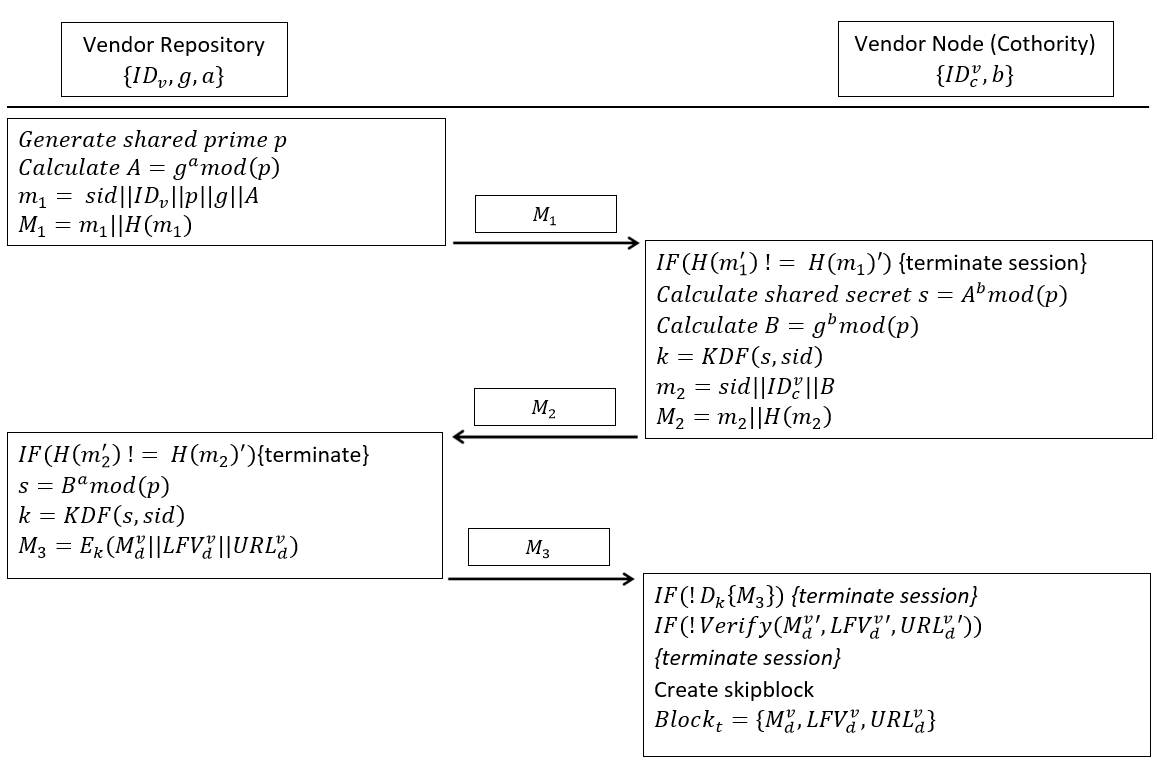
\includegraphics[width=1.0\textwidth]{figures/verification_process_protocol.png}
		\caption{Firmware update verification protocol} 
		\label{fig:verificationprocessprotocol}
	\end{center}
\end{figure}

\noindent \underline{\textbf{Step 1:}} $\text{Vendor Repository}\rightarrow\text{Vendor Node}$ \\
\indent Vendor repository \textit{v} will generate a shared prime \textit{p}, and calculate a shared number \textit{$A=g^a mod(p)$}. This shared number later will be used by vendor node to generate same shared secret. Vendor repository then create a message \textit{$m_1=(sid||ID_v||p||g||A)$}, then concatenate the message \textit{$m_1$} with the hash value of the message \textit{$H(m_1)$} and send it to the vendor node.

\noindent \underline{\textbf{Step 2:}} $\text{Vendor Node}\rightarrow\text{Vendor Repository}$ \\
\indent After receiving message \textit{$m_1'$} from vendor repository, vendor node will validate the message by applying the same hash function \textit{$H()$} to the message \textit{$m_1'$}. If the hashed-value do not match \textit{$H(m_1)'$}, vendor node will terminate the session. Once validated (\textit{$H(m_1')==H(m_1)'$}), vendor node will obtain session id \textit{sid'}, vendor repository's ID \textit{$ID_v'$}, shared prime \textit{p'}, shared base \textit{g'}, and shared number \textit{A'}. Next, vendor node calculate shared secret \textit{$s=A'^bmod(p')$} and shared number \textit{$B=g'^bmod(p')$}. Vendor node uses key derivation function \textit{$KDF()$}, passing shared secret \textit{$s$} and session id \textit{$sid$} as salt to create new session key \textit{$k$}. Vendor node then create a message \textit{$m_2=(sid||ID_c^v||B)$}, then concatenate the message \textit{$m_2$} with the hash value of the message \textit{$H(m_2)$} and send it to the vendor repository.

\noindent \underline{\textbf{Step 3:}} $\text{Vendor Repository}\rightarrow\text{Vendor Node}$ \\
\indent Once receive \textit{$m_2'$}, vendor repository will do the validation toward the message \textit{$m_2'$} and hashed-value \textit{$H(m_2)'$}. If the message is valid (\textit{$H(m_2')==H(m_2)'$}), vendor repository will obtain session id \textit{sid'}, vendor node's id \textit{$ID_c^{v'}$} and shared number \textit{B'} then calculate shared secret \textit{$s=B'^amod(p)$}. It will also use KDF to create same session key \textit{$k$}. Last, vendor repository encrypt message \textit{$m_3=E_k(M_d^v||LFV_d^v||URL_d^v)$} using symmetric encryption protocol with session key \textit{$k$}, then send the message \textit{$m_3$} back to vendor node.

\noindent \underline{\textbf{Step 4:}} $\text{Vendor Node}\rightarrow\text{Vendor Repository}$ \\
\indent Vendor node will decrypt the encrypted message \textit{$m_3'$} using its session key \textit{$k$}, and obtain the new firmware update metadata. Vendor node will broadcast the metadata to cothority member to be verified. Once the verifying process is done, vendor node will collect the signature from participated cothority member. The collected signature proof that the metadata has already verified, and ready to be put in the new skipchain block \textit{$BLOCK_t$}.

\subsection{Firmware Update Peer-to-Peer Verification Protocol}
\label{sec:p2pverificationprotocol}

Peer-to-peer verification protocol occurs between gateway \textit{$g$} and its belonging IoT device \textit{$d$}. This process is needed everytime gateway fetch new block data from the skipchain network (\textit{$URL_s$}). Each IoT device can verify if the firmware update notification from the gateway comes from a valid block from valid a skipchain network. The peer-to-peer verification protocol is shown in Figure \ref{fig:executionprocessprotocol1}.

\begin{figure}[H]
	\begin{center}
		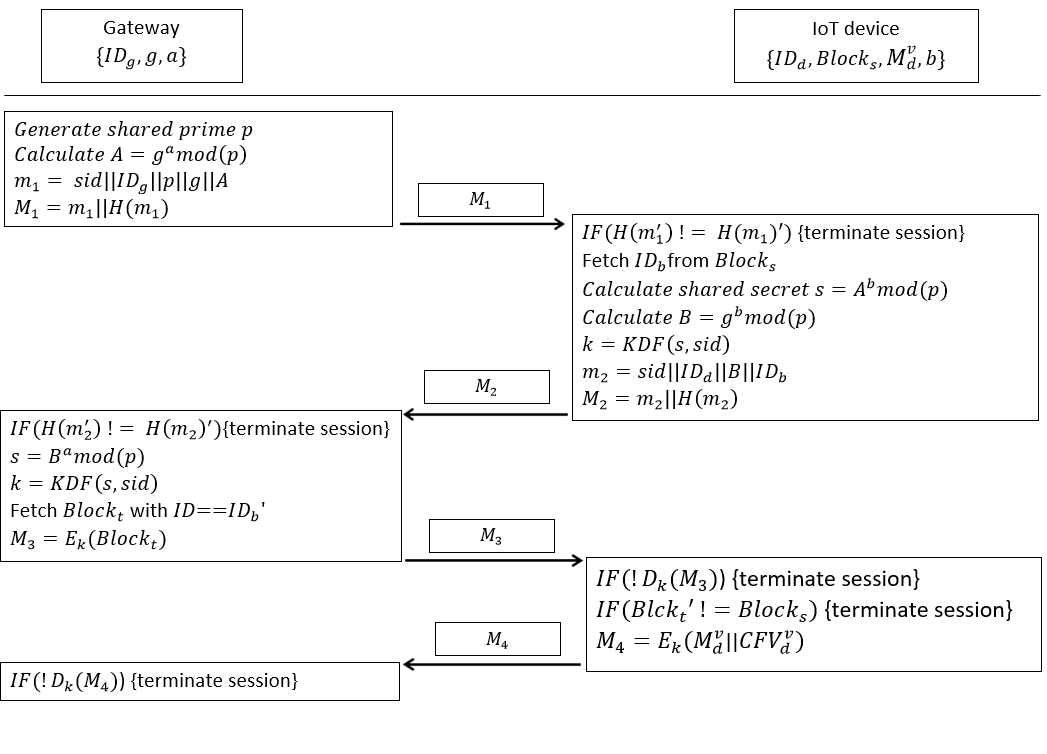
\includegraphics[width=1.0\textwidth]{figures/firmware_update_execution_1.png}
		\caption{Firmware update peer-to-peer verification protocol} 
		\label{fig:executionprocessprotocol1}
	\end{center}
\end{figure}

\noindent \underline{\textbf{Step 1:}} $\text{Gateway}\rightarrow\text{IoT Device}$ \\
\indent Gateway will generate a shared prime \textit{p}, and calculate a shared number \textit{$A=g^a mod(p)$}. Gateway then create a message \textit{$m_1=(sid||ID_v||p||g||A)$}, then concatenate the message \textit{$m_1$} with the hash value of the message \textit{$H(m_1)$} and send it to the IoT device.

\noindent \underline{\textbf{Step 2:}} $\text{IoT Device}\rightarrow\text{Gateway}$ \\
\indent Upon received message \textit{$m_1'$} from gateway, IoT device will validate the message by applying the same hash function \textit{$H()$} to the message \textit{$m_1'$}. If the hashed-value do not match \textit{$H(m_1)'$}, vendor node will terminate the session. Once validated (\textit{$H(m_1')==H(m_1)'$}), vendor node will obtain session id \textit{sid'}, gateway's id \textit{$ID_g'$}, shared prime \textit{p'}, shared base \textit{g'}, and shared number \textit{A'}. Next, IoT device calculate shared secret \textit{$s=A'^bmod(p')$} and shared number \textit{$B=g'^bmod(p')$}. IoT device uses key derivation function \textit{$KDF()$}, passing shared secret \textit{$s$} and session id \textit{$sid$} as salt to create new session key \textit{$k$}. IoT device then create a message \textit{$m_2=(sid||ID_d||B||ID_b)$}, then concatenate the message \textit{$m_2$} with the hash value of the message \textit{$H(m_2)$} and send it to the gateway.

\noindent \underline{\textbf{Step 3:}} $\text{Gateway}\rightarrow\text{IoT Device}$ \\
\indent Once receive \textit{$m_2'$}, gateway will do the validation toward the message \textit{$m_2'$} and hashed-value \textit{$H(m_2)'$}. If the message is valid (\textit{$H(m_2')==H(m_2)'$}), vendor repository will obtain session id \textit{sid'}, IoT device's id \textit{$ID_d^{v'}$}, skipblock id \textit{$ID_b'$} and shared number \textit{B'} then calculate shared secret \textit{$s=B'^amod(p)$}. It will also use KDF to create same session key \textit{$k$}. Gateway fetches the \textit{$BLOCK_t$} with id equals to \textit{$ID_b'$}. Last, gateway encrypt message \textit{$m_3=E_k(BLOCK_t)$} using symmetric encryption protocol with session key \textit{$k$}, then send the message \textit{$m_3$} back to IoT device.

\noindent \underline{\textbf{Step 4:}} $\text{IoT Device}\rightarrow\text{Gateway}$ \\
\indent IoT device will decrypt the encrypted message \textit{$m_3'$} using its session key \textit{$k$}, and obtain the new firmware update block. IoT device will verify the obtained \textit{$BLOCK_t'$} if it is matched with its pre-installed block \textit{$BLOCK_s$}. Once verified, IoT device encrypt its model information and current firmware version it has \textit{$m_4=E_k(M_d^v||CFV_d^v)$} using session key \textit{$k$}. Last, IoT device will send the message \textit{$m_4$} to the gateway.

\noindent \underline{\textbf{Step 5:}} \\
\indent Gateway will decrypt the message \textit{$m_4'$} and obtain model information \textit{$M_d^{v'}$} and current firmware version \textit{$CFV_d^{v'}$} of the IoT device \textit{d}. These information will be used for the next process, the firmware execution protocol in Section \ref{sec:executionprotocol}.

\subsection{Firmware Update Execution Protocol}
\label{sec:executionprotocol}

The firmware update execution will be processed once the peer-to-peer verification process is done. This process uses some variables collected from the peer-to-peer verification process, like session key \textit{$k$}, device model information \textit{$M_d^{v'}$} and device current firmware version \textit{$CFV_d^{v'}$}. With our assumption in Section \ref{sec:1_assumptions}, the IoT device will verify the firmware binary using its pre-installed public key of its vendor. The firmware update execution protocol is shown in Figure \ref{fig:executionprocess}.

\begin{figure}[H]
	\begin{center}
		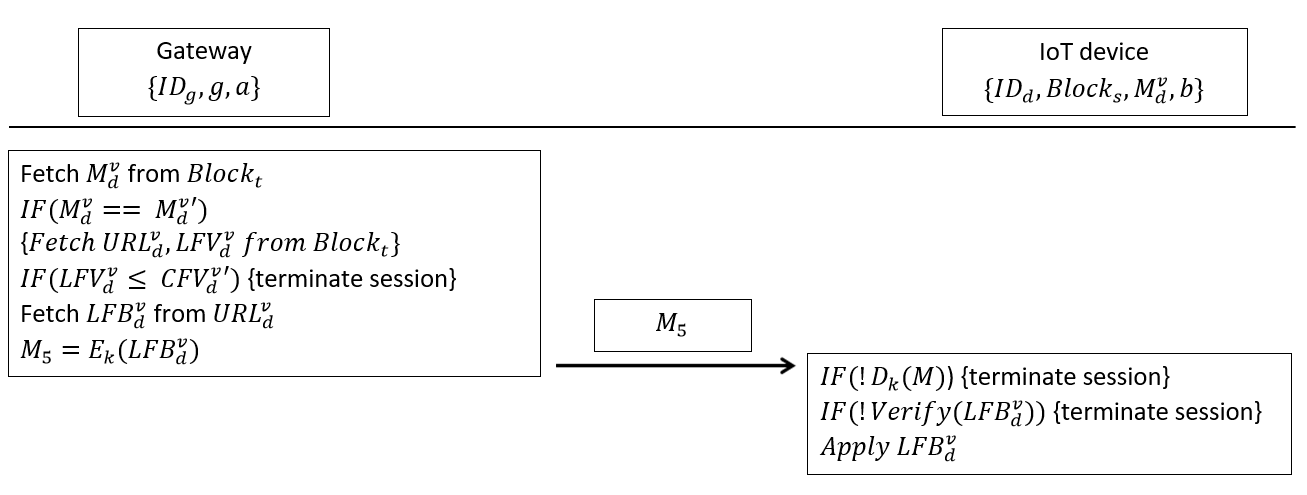
\includegraphics[width=1.0\textwidth]{figures/firmware_update_execution_2.png}
		\caption{Firmware update execution protocol} 
		\label{fig:executionprocessprotocol}
	\end{center}
\end{figure}

\noindent \underline{\textbf{Step 1:}} $\text{Gateway}\rightarrow\text{IoT Device}$ \\
\indent Gateway will fetch the target device model $M_d^v$ from the newly created block $BLOCK_t$. It will check if the targeted model device is same as the IoT device model $M_d^{v'}$ belonging to it. If there is targeted device model within its belonging IoT device ($M_d^v == M_d^{v'}$), it will fetch the download url $URL_d^v$ and the latest firmware version $LFV_d^v$ from the block $BLOCK_t$. Gateway will check if the latest firmware version is greater than the device current firmware version ($LFV_d^v \geq CFV_d^{v'}$). If the update is required, gateway will fetch the firmware binary $LFB_d^v$ from the download url $URL_d^v$. Last, gateway encrypt message $m_5=E_k(LFB_d^v)$ using session key $k$, then send the message $m_5$ to IoT device.

\noindent \underline{\textbf{Step 2:}} $\text{IoT Device}\rightarrow\text{Gateway}$ \\
\indent IoT device will decrypt the encrypted message \textit{$m_5'$} using its session key \textit{$k$}, and obtain the new firmware update binary. IoT device will verify the obtained \textit{$LFB_d^{v'}$} using its pre-installed vendor's public key. Once verified, IoT device will execute the firmware binary \textit{$LFB_d^{v'}$} and do the update process.